\chapter{Modelagem de Processo de Negócio}
\label{cp:bpmn}

Um processo de negócio é descrito por um ou mais procedimentos que, de modo conjunto, focam a realização de um objetivo de negócio. A execução de um processo de negócio possui condições muito bem definidas de início e término, e pode combinar procedimentos automáticos e/ou manuais~\cite{braghetto2011tecnicas}. 

Um processo de negócio pode ser modelado sob diferentes perspectivas. De acordo com os trabalhos sobre o assunto como~\citeauthoronline{russell2007foundations}~(\citeyear{russell2007foundations}),~\citeauthoronline{becker2000guidelines}~(\citeyear{becker2000guidelines}) e~\citeauthoronline{curtis1992process}~(\citeyear{curtis1992process}), as perspectivas mais relevantes são descritas a seguir~\cite{braghetto2011tecnicas}:

\begin{itemize}
\item \textbf{Controle de Fluxo}: descreve as tarefas pertencentes ao processo e sua ordem (parcial) de execução por meio de diferentes construtores de composição. As tarefas podem ser divididas em dois tipos: elementares (representando unidades atômicas de trabalho) e compostas (modularizando a ordem de execução de um conjunto de tarefas).

\item \textbf{Dados}: entrelaça dados da lógica do negócio ao controle de fluxo do processo. Esses dados podem ser documentos ou outros objetos que são passados de uma tarefa para outra, ou variáveis locais do processo usadas para expressar pré ou pós condições para a execução de uma tarefa.

\item \textbf{Organizacional (também chamada de recursos)}: atrela uma estrutura organizacional ao processo, por meio da definição de papéis (desempenhados por pessoas ou equipamentos) responsáveis pela execução das tarefas; 

\item \textbf{Tratamento de Exceções}: lida com as causas das exceções e as ações que precisam ser tomadas nos seus tratamentos.

\end{itemize}

Para a elaboração dos modelos de processos de negócio, é relevante o conhecimento de todos os elementos envolvidos na execução de processos, tais como atores, clientes internos e externos, recursos e limitações; por meio dos quais é estabelecido um modelo que propicia um melhor entendimento, organização e representação, seja esta uma visão contextual abstrata ou com alto nível de detalhamento, conforme necessário. 

Tipicamente, a representação de um modelo de processos inclui ícones, que representam atividades, eventos, decisões, condições e outros elementos do processo~\cite{brazil2011bpm}. Esses elementos podem conter informações sobre os relacionamentos entre eles e com o ambiente, bem como sobre o comportamento de cada elemento na cadeia de processos.

Neste trabalho, a \textit{Business Process Model and Notation} (BPMN) é utilizado como linguagem para a especificação do controle de fluxo de tarefas dos processos de negócio para a concepção de modelos que representem o plano de execução em experimentos controlados.

\section{\textit{Business Process Modeling and Notation}}

A especificação da notação BPMN foi elaborada e lançada em 2004 pelo Instituto de Gerenciamento de Processos de Negócio ou BPMI (\textit{Business Process Management Institute}), que realizou fusão ao Consórcio OMG. Posteriormente, a notação BPMN foi adotada pelo Consórcio OMG como o padrão para modelagem de processos. Após a padronização, foram lançadas algumas versões subsequentes, atualmente encontrando-se na versão 2.0~\cite{object2016business}.

A especificação agrega as melhores práticas da comunidade de modelagem de processos de negócio e os melhores conceitos existentes em outras notações relevantes, como as \textit{Event-Process Chains} (EPC) e os diagramas de atividades da \textit{Unified Modeling Language} (UML)~\cite{braghetto2011tecnicas}.

A construção de processos de negócio nessa notação utiliza um conjunto de padrões denominado ``metamodelo para definição de processos de negócio'' \cite{object2016business}. Esse metamodelo possui um conjunto principal de conceito que segundo ~\citeauthoronline{Weske2012}~(\citeyear{Weske2012}) são descritos nas seguintes categorias:

\begin{itemize}
\item \textbf{Modelo de Processo}: um modelo de processo representa um diagrama para um conjunto de instâncias de processos com uma estrutura similar. Cada modelo consiste em um conjunto de nós e arestas direcionadas com o objetivo de representar uma dada atividade. Permite-se aninhar modelos de processos dentre de outros modelos de processos, porém tal prática facilmente eleva o nível de complexidade.

\item \textbf{Arestas}: consistem em arestas direcionadas que expressam algum tipo de relacionamento intra ou inter-procedural.
\item \textbf{Nós}: um nó em modelo de processo pode representar uma atividade, um evento ou um portão.
\begin{tasks}
	\task \textit{Atividades}(\textit{Activity Model}): cada atividade descreve uma unidade de trabalho conduzida em um processo de negócio, podendo aparecer uma ou mais vezes em um mesmo modelo de processo. Uma atividade não objetiva dividir ou juntar nós, mas sim a execução de atividade, a qual possui uma entrada (aresta de entrada) e saída (aresta de saída).
	\task \textit{Eventos}(\textit{Event Model}): os eventos capturam a ocorrência de estados relevantes para o processo de negócio. Os eventos sempre estão presentes em modelos de processo, e são estes que o devem iniciar e finalizar.
	\task \textit{Portões}(\textit{Gateway Model}): um portão é utilizado para expressar o controle de fluxo, adicionando sequências, dividindo ou juntando nós.
\end{tasks}

\end{itemize}

Na Figura~\ref{image:metamodelo} são apresentadas as relações de hierarquia e de interação entre os elementos do metamodelo descrito anteriormente.

\begin{figure}[!ht]
\centering
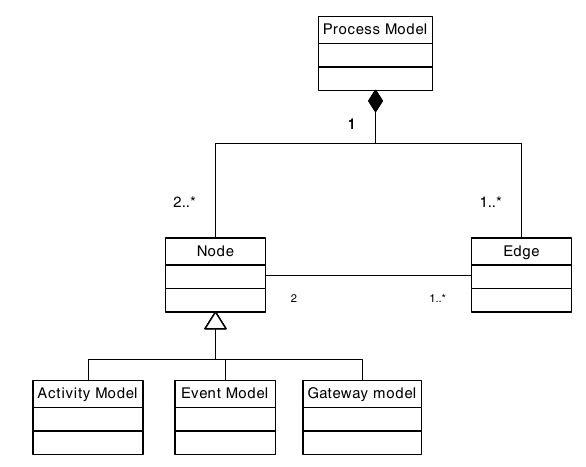
\includegraphics[width=0.7\textwidth]{images/metamodelo.png}
\caption{Metamodelo da modelagem de processo de negócio~\cite{Weske2012}.}
\label{image:metamodelo}
\end{figure}

Segundo~\citeauthoronline{correia2015enhancing}~(\citeyear{correia2015enhancing}), \textit{Business Process Modeling and Notation} (BPMN) é atualmente a notação de modelagem de processos de negócio mais usada entre profissionais da área, devido  a sua flexibilidade e abrangência. Consiste em uma tecnologia recente e pode ser utilizada por profissionais com diferentes níveis de conhecimento técnico. A formalização dos conceitos de modelagem de processos de negócio é baseada em um metamodelo construído a partir da linguagem \textit{Unified Modeling Language} (UML). 

Nesse sentido, a especificação \textit{BPMN} também provê uma notação gráfica para representar processos de negócio por meio de um diagrama chamado ``diagrama de processo de negócio''. Esse diagrama é elaborado a partir de um conjunto de elementos gráficos que compõem diagramas simples de serem desenvolvidos e
compreendidos. 

\begin{figure}[!ht]
\centering
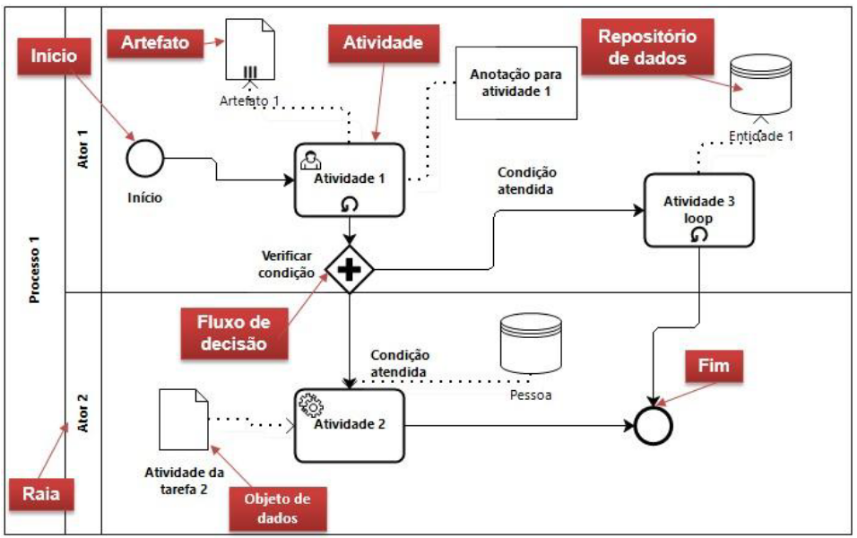
\includegraphics[width=0.97\textwidth]{images/diagrama.png}
\caption{Exemplo de diagrama BPMN -- adaptado de \cite{Weske2012}.}
\label{diag}
\end{figure}

Na Figura~\ref{diag} é apresentado, como exemplo, um simples diagrama de processo de negócio, no qual é possível identificar a interação entre dois atores por meio da execução de atividades e trocas de mensagens, assim como, o uso de recursos como artefatos e repositórios de dados. Cada elemento da notação BPMN é identificado pelas notas em vermelho.

A especificação completa da atual versão divide seus elementos em quatro categorias básicas: objetos de fluxo (\textit{Flow Objects}), objetos de conexão (\textit{Connecting Objects}), vias (\textit{Swimlanes}) e artefatos (\textit{Artifacts}). 
Na Figura~\ref{img:elementos} há uma visão geral dos elementos da atual versão do \textit{BPMN}.

\begin{figure}[!ht]
\centering
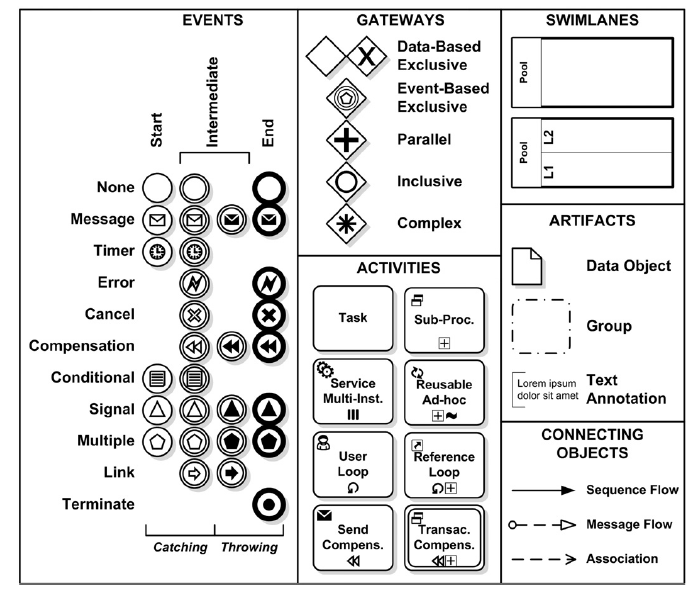
\includegraphics[width=\textwidth]{images/elementos.png}
\caption{Conjunto de elementos que compõem a versão BPMN 2.0~\cite{object2016business}.}
\label{img:elementos}
\end{figure}

\section{Protocolos de experimentação usando BPM}

A compreensão do projeto do experimento e revisar suas informações é fundamental não só para a execução do experimento, mas também para sua replicação. Diversos pesquisadores têm realizado projetos pilotos que ocasionam  possíveis erros e incorrendo em aumento de custos~\cite{Kitchenham2008}. 

A utilização da notação de processo de negócio pode contribuir diretamente tanto na concepção quanto na execução do protocolo de estudo experimental. Primeiramente, devido à facilidade de compreensão do uso que compõem a respectiva notação, principalmente por ser baseado em um padrão~\textit{UML}. Em segundo ponto, a utilização de pacotes de laboratório para o armazenamento das informações relativas aos protocolos realizados em cada experimento.

A representação do modelo de diagrama de processo de negócio também deve ser incorporada ao pacote de laboratório, viabilizando o compartilhamento do protocolo juntamente com os dados referentes ao experimento, tais como hipóteses, variáveis dependentes e independentes entre outros, permitindo, desse modo, atrelar os artefatos do experimento às suas respectivas atividades, seja em relação de saída (atividade na qual o artefato é produzido) ou em uma relação de entrada (atividade na qual o artefato é consumido).

A elaboração do conjunto de atividades, que compõem o protocolo de experimentação, deve contemplar todas as fases do processo experimental, como definido na Seção~\ref{sect:processoexperimentacao}, apresentando as seguintes fases: \textit{Definição}, \textit{Planejamento}, \textit{Operação}, \textit{Análise e Interpretação}, e por fim, \textit{Empacotamento}. Cada fase deve conter seu respectivo conjunto de atividades e a produção de artefatos que são incorporados ao corpo do experimento.

A seguir, nas figuras~\ref{img:modelo-definicao},~\ref{img:modelo-planejamento},~\ref{selecao},~\ref{g1},~\ref{g2} e~\ref{img:modelo-analise} são apresentados comparativos entre o modelo proposto de fases do processo experimental e a condução do experimento executado no trabalho de~\citeauthoronline{martins2017modeluiviz} (\citeyear{martins2017modeluiviz}).


Inicialmente, na Figura~\ref{img:modelo-definicao} é apresentado o modelo de processo de negócio da Fase de Definição, representada pela Figura~\ref{image:definicao}, na qual são apresentadas atividades que visam a definição aspectos relativos à problemática e ao contexto do experimento em questão. Nesse caso em específico, são realizadas atividades relativas à definição e à declaração do problema, e também, definição do contexto, resultando nos artefatos apresentados pelos elementos de dados (\textit{Data Object}).

%%%%%%%%%%%%fase de definição
\begin{figure}[!ht]
\centering
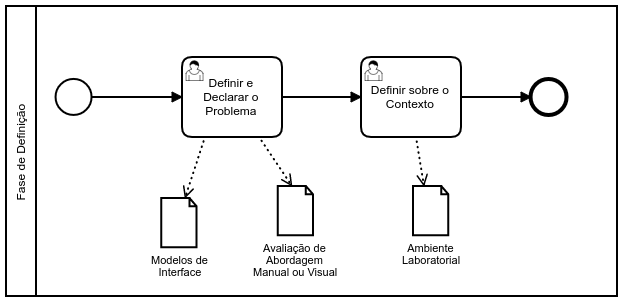
\includegraphics[width=0.95\textwidth]{images/modelo-definicao.png}
\caption{Modelo de processo de negócio referente a Fase de Definição.}
\label{img:modelo-definicao}
\end{figure}

Na etapa seguinte, a fase de \textit{Planejamento} (Figura~\ref{img:modelo-planejamento}) apresenta no modelo de processo são especificados diversos elementos importantes em estudo experimental, como hipóteses, variáveis, participantes, conforme a Figura~\ref{image:planejamento}. 

%%%%%%%%%%% fase de planejamento
\begin{figure}[!ht]
\centering
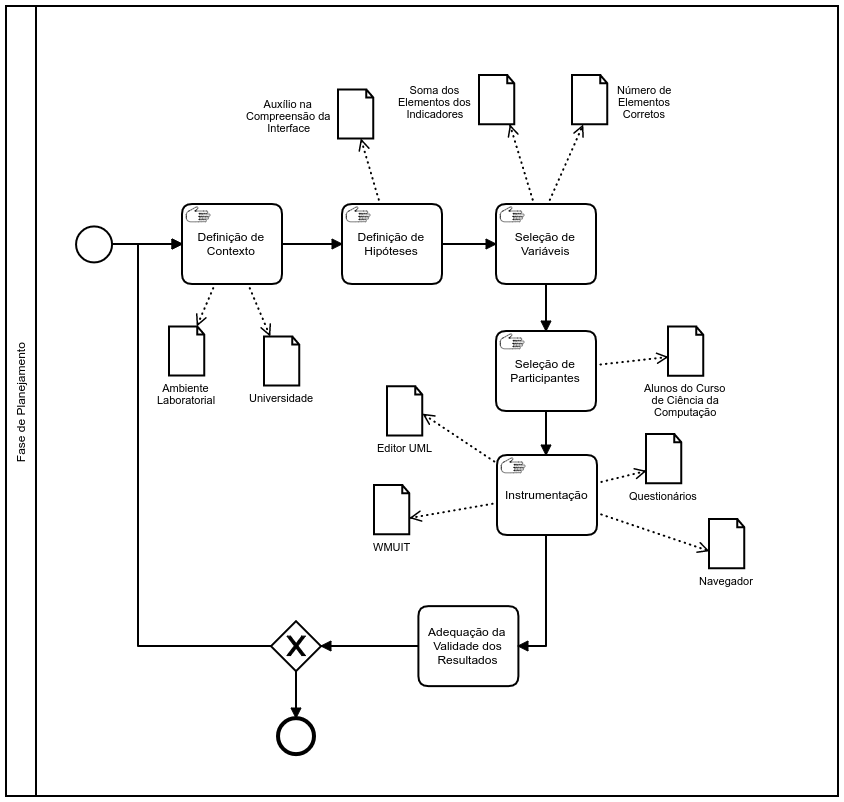
\includegraphics[width=\textwidth]{images/modelo-planejamento.png}
\caption{Modelo de processo de negócio referente a Fase de Planejamento.}
\label{img:modelo-planejamento}
\end{figure}

As Figuras~\ref{selecao},~\ref{g1} e~\ref{g2} são referentes à fase de \textit{Operação}, definida na Figura~\ref{image:operacao}. Esta fase, como pode ser observado pelo modelo de processo de negócio, é a mais específica para cada processo experimentação, cujas atividades são altamente dependentes das definições anteriores.

Como ilustrado na Figura~\ref{selecao}, a partir do conjunto de participantes foi proposta uma separação em dois grupos, os quais deveriam cumprir o mesmo conjunto de atividades de modo intercalado. Nas figuras~\ref{g1} e~\ref{g2} são apresentam as atividades de cada grupo, as quais devem ser concomitantes, de modo a utilizar as duas abordagens propostas e prover dados para posterior avaliação das hipóteses.

%%%%%%%fase de operação
%%%%%%%%%%%%%% selecao grupos
\begin{figure}[!ht]
\centering
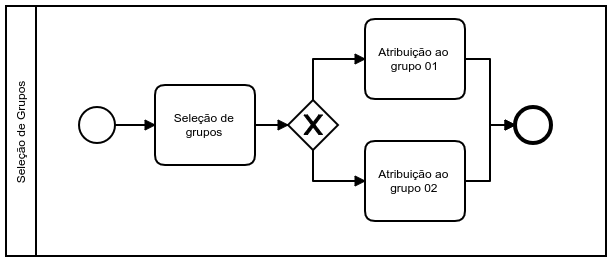
\includegraphics[width=0.7\textwidth]{images/selecao.png}
\caption{Atribuição de participantes aos grupos.}
\label{selecao}
\end{figure}


\begin{landscape}

%%%%%%%%%%%%%% grupo 01
\begin{figure}[!ht]
\centering
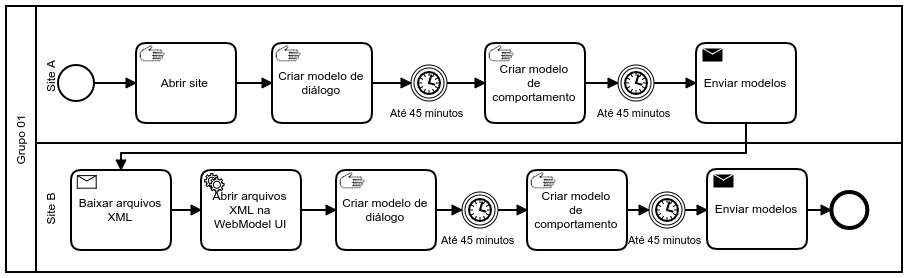
\includegraphics[scale=0.63]{images/grupo01.png}
\caption{Diagrama BPM referente às atividades dos participantes do primeiro grupo.}
\label{g1}
\end{figure}




%%%%%%%%%%%%%%% grupo 02
\begin{figure}[!ht]
\centering
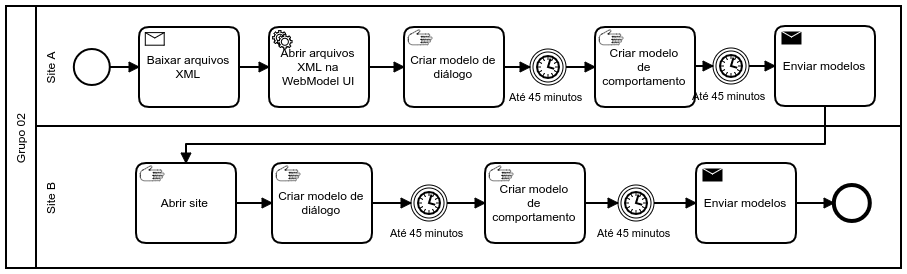
\includegraphics[scale=0.63]{images/grupo02.png}
\caption{Diagrama BPM referente às atividades dos participantes do segundo grupo.}
\label{g2}
\end{figure}


\end{landscape}


%%%%%%%%%analise
Por fim, na Figura~\ref{img:modelo-analise} e Figura~\ref{image:analise}, pode-se observar as atividades da fase de \textit{Análise e Interpretação} para o referido estudo experimental. Nesse caso em específico, a partir dos dados coletados na etapa anterior, são aplicados modelos estatísticos, seguido de uma redução do conjunto de dados, permitindo a eliminação de vieses e avaliação das hipóteses. A partir dos resultados são elaboradas as conclusões do estudo e suas respectivas recomendações. De forma paralela, todo o conjunto de dados e informações é registrado em um pacote de laboratório.

\begin{figure}[!ht]
\centering
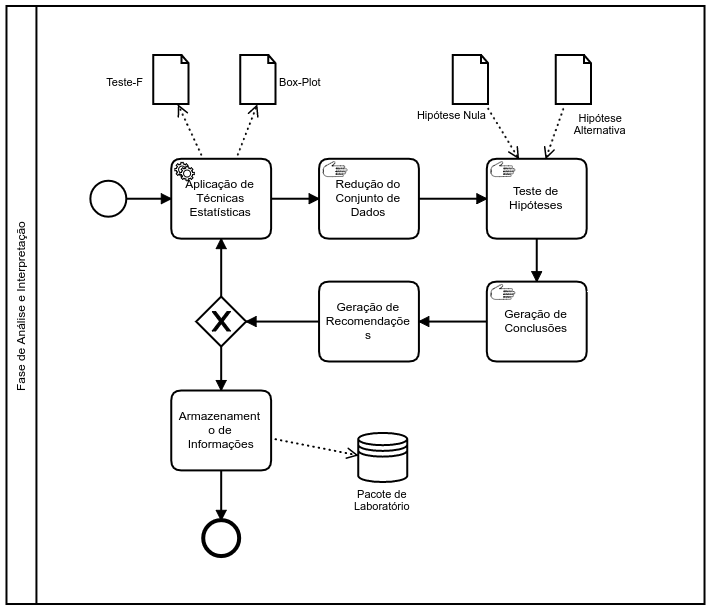
\includegraphics[width=\textwidth]{images/modelo-analise.png}
\caption{Modelo de processo de negócio referente a Fase de Análise e Interpretação.}
\label{img:modelo-analise}
\end{figure}

\section{Considerações Finais}
Neste capítulo foi apresentado uma visão geral em relação a modelagem de processos de negócio, em especial, utilizando a notação BPMN, assim como, a elaboração de protocolos de execução em experimentos controlados. Um modelo processo pode ser elaborado sob diferentes perspectivas, tais como a perspectiva de controle de fluxo, perspectiva de dados, perspectiva organizacional e perspectiva de tratamento de exceções; as quais diferem a partir do ambiente e do conjunto de conhecimento sobre o processo a ser modelado. Dentre as notações utilizadas, tem-se destaque para a \textit{Business Process Modeling and Notation}, presente no arcabouço de notações UML e muito utilizada tanto para âmbito pesquisa quanto empresarial.

Na Engenharia de Software Experimental, pacotes de laboratório têm sido utilizados são compartilhados entre grupos de pesquisa. Porém foram detectadas ausências de informações relativas ao plano de execução do experimento, para isto é proposta a utilização da notação BPMN para a representação do conjunto de atividades executadas em cada fase do processo experimental.

No próximo capítulo, é apresentada a ferramenta de construção de protocolos de execução em experimentos controlados, a qual se utiliza da notação BPMN para modelagem e vincula estes dados em pacotes de laboratório definidos a partir da \textit{ExperOntology}.






